% !TEX root = ../main.tex
% !TEX program = xelatex
\section{数据预处理与探索性分析}
\subsection{数据预处理}
本文数据来自赛题附件，涵盖负载、光伏、电价及不同时间发布的光伏预报。各附件的时间写法和排列方式有所不同，功率数据也需要转换为调度使用的电量。为使各项数据准确对应，进行以下处理。

\noindent\textbf{1．检查缺失与异常记录。}原表已有记录未发现空单元格，但按实际时间排列后，全年实测数据缺少1月1日00:00—00:10这一段，启动处理见第6.3节。夜间光伏为零属于正常情况，予以保留；极端取值经原表核对后，也不因数值较大或较小而直接删除。

\noindent\textbf{2．统一时间与区间对应关系。}各行数据用于标注时刻开始的10分钟区间。例如，首行“00:10”对应00:10—00:20，末行“00:00+1”对应次日00:00—00:10。问题一中，每天各时段的负载、光伏出力和电价均相同，因此将末行零点数据放到当天开头；全年连续数据则按实际日期衔接，不将次日零点移回当天。描述性统计仍按原表日期分组。

\noindent\textbf{3．区分预报批次。}统一日期与时间格式，并为光伏预报同时保留“发布时间”和“目标时刻”，避免新预报覆盖旧预报。超出实测覆盖范围的预报予以保留，但不参与误差比较。

\noindent\textbf{4．转换电量并核对。}每个时段为10分钟，即 $\Delta t=1/6\ \mathrm h$，将功率按 $E=P\Delta t$ 转换为电量，并核对整理前后的数值及时间对应关系。全年统计用于识别数据特征，逐日决策仅使用当时已获得的信息。

\subsection{探索性分析}
经过整理与分析，得到以下四点发现。

\subsubsection*{（1）光伏富余与用电缺口存在时间错位}

代表日午间光伏能够覆盖负载并产生富余，傍晚光伏回落后，外网需要补足的电量明显增加，且与较高电价有所重合。全年有330天出现过光伏功率高于负载的情况，说明光伏富余具有普遍性。

因此，储能需要将富余光伏或低价购电留到后续使用。能够转移多少电量，又受到容量、充放电功率和效率限制。这说明购电与储能应当按时段联合安排，全天电量总和不能代替逐时供需判断。

\subsubsection*{（2）负载与光伏的年内变化不同步}

\begin{figure}[htbp]
\centering
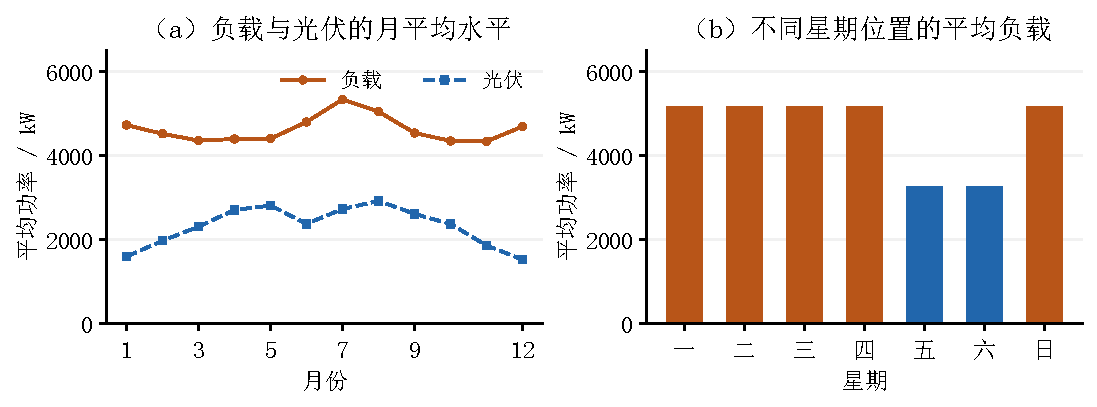
\includegraphics[width=\textwidth]{fig/data_compact.pdf}
\caption{负载与光伏的季节差异及负载的星期规律}
\label{fig:data_compact}
\end{figure}

图~\ref{fig:data_compact}(a)显示，夏季负载较高，光伏也能提供较多电量；冬季负载虽有所回落，光伏下降却更加明显。以月平均功率差衡量，12月负载减去光伏约为3177 kW，接近5月的两倍。

这表明，\textbf{外网补电压力取决于负载与光伏的共同变化}。不同月份的电价也存在差异，因此需要随近期数据更新判断，不能将代表日的购电安排直接复制到全年。

\FloatBarrier
\subsubsection*{（3）负载具有星期规律，光伏与电价的日际变化更强}

图~\ref{fig:data_compact}(b)显示，按实际星期分组后，周五、周六的平均负载比其余五天低约36.8\%；负载与一周前数据的相关性也高于与前一天数据的相关性。因此，同一星期位置的历史负载更有参考价值。

光伏在不同日期呈现相似的昼夜变化，但扣除各月相同时刻的平均水平后，其一周相关性接近于零。这说明，光伏的相似性主要来自白天发电、夜间为零的共同特征，负载的星期规律不宜直接用于光伏预测。

相同时刻在不同日期的电价也存在较大差异。由此，负载、光伏和电价应分别利用适合自身特点的历史信息，再共同参与购电决策。

\subsubsection*{（4）日内新预报提高预测精度，为滚动调整提供依据}

\begin{figure}[H]
\centering
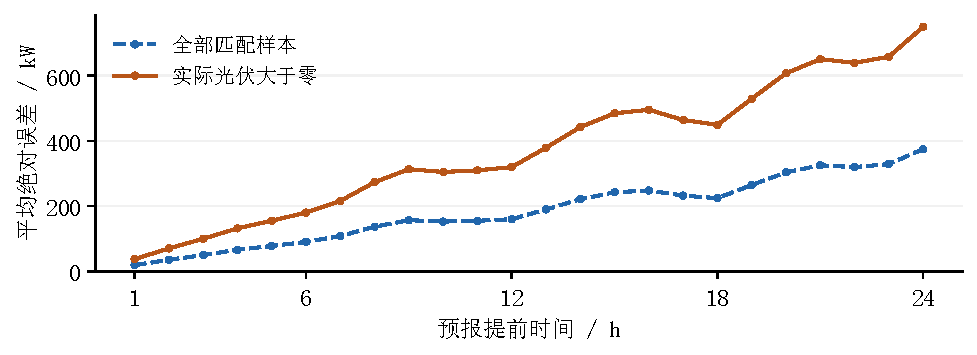
\includegraphics[width=0.78\textwidth]{fig/forecast_compact.pdf}
\caption{光伏预报提前时间与平均绝对误差}
\label{fig:forecast_compact}
\end{figure}

将不同发布时间的预报与相同目标时刻的实测值匹配后发现，预报提前时间越长，平均绝对误差总体越大，如图~\ref{fig:forecast_compact}所示。在实际光伏大于零的4177组配对样本中，使用目标时刻前最新日内预报后，平均绝对误差由约378.8 kW降至116.3 kW，下降约69\%。

新预报为修正购电提供了更准确的信息。考虑到约17.4\%的样本更新后误差增大，且修改订单需要付费，后续由优化模型综合预报、储能余量和调整成本决定改单幅度，将预测精度的改善转化为实际购电收益。
